\documentclass{llncs}

\usepackage{graphicx}

%\usepackage{caption, subcaption}
%\captionsetup{compatibility=false}
\usepackage[caption=false]{subfig}

\makeatletter%
\newbox\sf@box%
\newenvironment{SubFloat}[2][]%
{\def\sf@one{#1}%
	\def\sf@two{#2}%
	\setbox\sf@box\hbox%
	\bgroup}%
{ \egroup%
	\ifx\@empty\sf@two\@empty\relax%
	\def\sf@two{\@empty}%
	\fi%
	\ifx\@empty\sf@one\@empty\relax%
	\subfloat[\sf@two]{\box\sf@box}%
	\else%
	\subfloat[\sf@one][\sf@two]{\box\sf@box}%
	\fi%
}%
\makeatother%

\usepackage{url}
\usepackage{courier}
\usepackage{listings}

\usepackage{pifont}

\usepackage{xcolor}
\definecolor{mygreen}{rgb}{0,0.5,0}
\definecolor{mypurple}{rgb}{0.5,0,0.33}

%!TEX root = ./paper1.tex

\lstset{
  float=tb,
	captionpos=b,
	breaklines=true,
	xleftmargin=20pt,
	basicstyle=\ttfamily\scriptsize,
	numberstyle=\tiny,
	flexiblecolumns=true,
	numbers=left,
	nolol=false,
	tabsize=2
}

\lstdefinelanguage{OCL}{
morekeywords={import,if,then,else,endif,self,and,true,false,def,includes,OclElement,package,let,in},
sensitive=true,
morecomment=[l]{--},
morestring=[b]",
morestring=[b]',
showstringspaces=false
}

\lstdefinelanguage{QVTo}{
morekeywords={import,modeltype,uses,transformation,inout,in,out,configuration,property,main,var,if,then,else,endif,map,new,self,library,helper, mapping, and,return, when, where, object, true, false, result},
sensitive=true,
morecomment=[l]{--},
morecomment=[l]{//},
morestring=[b]",
morestring=[b]',
showstringspaces=false
}

\lstdefinelanguage{Acceleo}{
morekeywords={template, file, if, else, for},
sensitive=true,
morecomment=[l]{--},
morecomment=[l]{//},
morestring=[b]",
morestring=[b]',
showstringspaces=false
}

\lstdefinelanguage{MWE}{
morekeywords={module, import, var, true, false, },
sensitive=true,
morecomment=[l]{//},
morestring=[b]",
showstringspaces=false
}

\lstdefinelanguage{Java}{
morekeywords={class, private, public, true, false, new, if, for, int, return, void, extends, implements, this, null, super, import, package},
sensitive=true,
morecomment=[l]{//},
morestring=[b]",
showstringspaces=false
}

\lstdefinelanguage{JastAdd}{
morekeywords={abstract, ast, syn, inh, eq, boolean, int, false, true, if, for, return},
morestring=[b]',
sensitive=true
}

\lstdefinelanguage{NaBL}{
morekeywords={rules, defines, unique, non, refers, to},
sensitive=true
}

\lstdefinelanguage{Gra2Mol}{
morekeywords={rule, from, to, queries, mappings, skip, end_rule},
morestring=[b]',
sensitive=true
}

\lstdefinelanguage{Xtext}{
morekeywords={terminal, returns, grammar, import, fragment, current},
morestring=[b]',
sensitive=true
}

\lstdefinelanguage{Xtend}{
morekeywords={FOR, ENDFOR, IF, ELSE, ENDIF, def, protected, void, new, var, typeof, return},
morestring=[b]',
morestring=[b]",
morecomment=[s]{/*}{*/}
sensitive=true
}




\lstset{% general command to set parameter(s)
	%basicstyle=\scriptsize,%\libertineDisplay, % print whole listing small
	keywordstyle=\bfseries\color{mypurple},	% underlined bold black keywords
	keywordstyle=[2]\bfseries\textsl,	% slanted directives
	commentstyle=\color{mygreen}\textit, % white comments
	%stringstyle=\ttfamily, % typewriter type for strings
	showstringspaces=false,	% no special string spaces
	breaklines=true,	% break lines
	breakatwhitespace=false,
	escapechar=@,	% escape character for latex, e.g. \label{key}
	numberbychapter=false
}

\addtolength{\intextsep}{-15pt}
\addtolength{\textfloatsep}{-15pt}


\begin{document}

%opening
\title{A Domain Specific Transformation Language to Bridge Concrete and Abstract Syntax}

\author{Adolfo S\'{a}nchez-Barbudo Herrera\inst{1}, Edward D. Willink\inst{2},
Richard F. Paige\inst{1}}

\institute{
Department of Computer Science, University of York, UK.\\
\email{\{asbh500, richard.paige\}\_at\_york.ac.uk}
\and 
Willink Transformations Ltd. 
\email{ed\_at\_willink.me.uk}
}
\maketitle

\begin{abstract}
%In Model-Driven Engineering, there are modelling languages where the gap between concrete syntax (CS) and abstract syntax (AS) is so significant that providing tools to create and manage valid models is a non-trivial task. 
Existing language workbenches, such as Xtext, support bridging the gap between the concrete syntax (CS) and abstract syntax (AS) of textual languages. However, the specification artefacts -- i.e. grammars -- are not sufficiently expressive to completely model the required CS-to-AS mapping, when it requires complex name resolution or multi-way mappings. This paper proposes a new declarative domain specific transformation language (DSTL) which provides support for complex CS-to-AS mappings, including features for name resolution and CS disambiguation. We justify the value of and need for a DSTL, analyse the challenges for using it to support mappings for complex languages such as Object Constraint Language, and demonstrate how it addresses these challenges. We present a comparison between the new DSTL and the state-of-the-art Gra2Mol, including performance data showing a significant improvement in terms of execution time.

\keywords{
Concrete Syntax 
$\cdot$ Abstract Syntax
$\cdot$ Domain Specific Transformation Language
$\cdot$ Xtext
$\cdot$ OCL
$\cdot$ Gra2Mol}
\end{abstract}

\section{Introduction}

%In Model-Driven Engineering (MDE), models are the first class artefacts managed by end users for different engineering purposes (e.g., software development, re-engineering, process design, documentation). Models can be expressed in varied forms (e.g. text, diagrams, spreadsheets) conforming to the concrete syntax (CS) of the language. Regardless of the specific language CS, the tools provided for the modelling languages manipulate models that conform to its abstract syntax (AS), or meta-model. 
One of the challenges that Model-Driven Engineering (MDE) tool implementors face when creating modelling languages is how to effectively bridge the gap between the concrete syntax (CS) and the abstract syntax (AS) of a language: the CS must be designed so that end-users have a familiar and accessible syntax, whereas the AS must be provided behind-the-scenes to enable model management and manipulation -- and the two artefacts must be related.

Although this is a general challenge addressed by many works in the field, there are still gaps, particularly for bridging the CS-to-AS (CS2AS) gap for non-trivial modelling languages like the Object Constraint Language (OCL). %To adequately introduce this gap, we firstly describe the motivation and scope, focusing on the technical challenges of building the official Eclipse OCL tools. To conclude the introductory section, we clarify the contributions of this paper, and its overall structure.
To understand the aims of this research, we introduce its scope and motivation in the remainder of this section. Section~\ref{sec:problem} goes deeper into the challenges that arise when specifying CS2AS bridges for languages like OCL. Section~\ref{sec:solution} introduces the proposed solution to overcome these challenges. Section~\ref{sec:relatedWork} assesses related work, and we present a more extensive comparative study with Gra2Mol in Sect.~\ref{sec:gra2mol}. We give final remarks and future work in Sect.~\ref{sec:futureWork} and conclude in Sect.~\ref{sec:conclusions}.

\subsection{Scope}
\label{subsec:scope}

Bridging the CS and the AS of a modelling language is a topic with significant related work (discussed in Sect.~\ref{sec:relatedWork}).
We focus on the problem for a subset of languages:
\begin{itemize}
\item Those whose AS is given in the form of an established (possibly standardised) meta-model. In other words, the end user is interested in editing models conforming to an already existent meta-model.% Examples might include OMG standard metamodels, which are widely deployed and used.
\item Those whose CS is textual and given in the form of a grammar. Although we are aware of previous work \cite{jouault2006tcs,heidenreich2011emfText,voelter2011mps} that supports for textual concrete syntaxes without any grammar provision, they are out of this paper scope. %as they target a different class of problem.
\end{itemize}

We use OCL~\cite{omg2014ocl} to illustrate the ideas of our approach. OCL has a textual CS and managing instances of it consists of editing models conforming to the language AS (meta-model). The grammar and meta-model come from the specification defined by the Object Management Group (OMG).

%[?]. Should I mention EMF as modeling platform ?
%TODO. This work is a continuation of the work presented at the Ocl workshop


\subsection{Motivation}
\label{subsec:motivation}

%With respect to the topic of bridging the gap between a textual CS (defined by a grammar) and an AS (defined by a meta-model), many publications and open tools might be found [????].
To clarify the motivation for our approach, we expose a problem with a specific language workbench: Xtext~\cite{eysholdt2010Xtext}. Then, we briefly introduce our solution.

%\textbf{Problem.} Xtext is a language workbench which gives you support to textual modelling languages in the form of generating a parser capable of producing AS models. For the sake of bridging the CS and AS of a language, Xtext specification artefacts, i.e. the grammars, let us specify those bridges.


%\begin{lstlisting}[caption=Xtext grammar excerpt, label=lst:XtextExcerpt, language=Xtext]
%import MM 'http://myMetamodelNSURI';
%TopRule returns Model: // grammar non-terminal -> returns Model AS Class
%  'model'        // grammar terminal (Keyword)
%    (element+=   // matches Model::element AS Property
%      Element)*; // grammar non-terminal reference
%SubRule returns Element:        // grammar non-terminal -> returns Element AS Class 
%  'element'      // grammar terminal (Keyword)
%    name=        // matches Element::name AS Property
%      ID;        // grammar terminal reference
%\end{lstlisting} 

%Listing~\ref{lst:XtextExcerpt} shows how an Xtext grammar that imports an existing meta-model (AS), uses some EBNF like constructs to define the CS, but also incorporates additional syntax to map the CS and the AS. In particular:
%\begin{itemize}
%\item Lines 2 and 6 map grammar non-terminals with meta-model classes, respectively Model and Element.
%\item Line 4 maps the consumption of non-terminals with a property of the Model meta-model class.
%\item Line 8 maps the consumption of a terminal with a property of the Element meta-model class.
%\end{itemize}

\textbf{Problem.} Xtext grammars provide the means to specify bridges between the CS and the AS. However, this can only be done easily for simple languages. Consider the following example of an OCL expression: % that will be used along the paper:

\begin{lstlisting}[label=lst:namedExp, language=Xtext]
x.y
\end{lstlisting} 

Fig.~\ref{fig:ExampleCS} shows a plausible CS definition. It uses a very simplified OCL grammar and CS with just navigation expressions for ease of presentation.

%\begin{figure}[htbp]
%	\centering
%	\begin{subfigure}{0.35\textwidth}
%		\centering
%		\begin{lstlisting}[label=lst:ExampleGrammar, language=Xtext]
%NameExpCS:
%  sName=SimpleNameCS 
%  ( navOp=('.' | '->')
%    navExp=NameExpCS)?;
%SimpleNameCS:
%  name=(ID | 'self');
%		\end{lstlisting} 
%	\end{subfigure}%
%	\begin{subfigure}{0.65\textwidth}
%		\centering
%		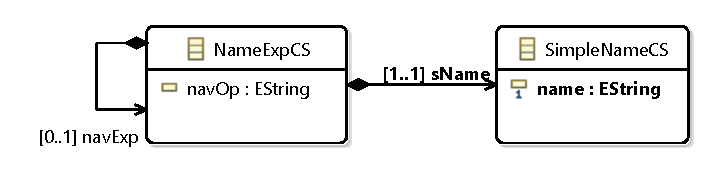
\includegraphics[width=\textwidth]{images/NameExpCS.pdf}
%	\end{subfigure}
%	\caption{Example CS definition}
%	\label{fig:ExampleCS}
%\end{figure}
\begin{figure}[htbp]
  \captionsetup[subfigure]{labelformat=empty}
  \begin{SubFloat}[]{}%
  	\begin{minipage}{0.35\textwidth}%
    \begin{lstlisting}[label=lst:ExampleGrammar, language=Xtext]
NameExpCS:
  sName=SimpleNameCS 
  ( navOp=('.' | '->')
  navExp=NameExpCS)?;
SimpleNameCS:
  name=(ID | 'self');
    \end{lstlisting} 
    \end{minipage}
  \end{SubFloat}
  %\hfill
  \begin{SubFloat}[]{}%
    \begin{minipage}{.60\textwidth}%
	  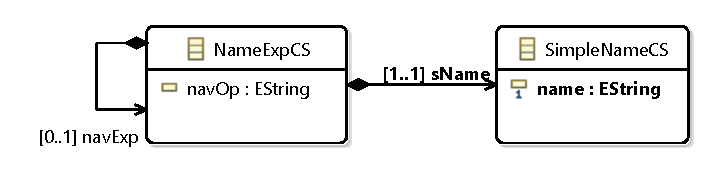
\includegraphics[width=\textwidth]{images/NameExpCS.pdf}
    \end{minipage}
  \end{SubFloat}
  %	\subfloat[]{\includegraphics[width=0.45\textwidth]
  %				    {images/NameExpCS.pdf}
  %	}
  \caption{Example CS definition}
  \label{fig:ExampleCS}
\end{figure}

In terms of AS (Clause 8 of~\cite{omg2014ocl}), we can be sure that \textit{'y'} must be a \textit{PropertyCallExp}. This means, in terms of evaluation (dynamic semantics), that the \textit{'y'} property must be navigated from the object evaluated from the \textit{PropertyCallExp} source (i.e. \textit{'x'}). \textit{'x'} could be a \textit{VariableExp}, whose evaluation uses the value of the \textit{'x'} variable (perhaps defined in an outer \textit{LetExp}). However, in OCL, \textit{'x'} could also be another property navigation using the value of the implicit \textit{'self'} variable. In other words, the original expression could be shorthand for \textit{'self.x.y'}.

This kind of situation cannot be handled by Xtext grammars. Syntactically, it is unknown whether the name \textit{'x'} that precedes the \textit{'.'} operator is a \textit{VariableExp}, or a \textit{PropertyCallExp}. Additional semantic information (static semantics) is required. Despite enhancing EBNF notation~\cite{wirth1996ebnf} to map the AS from the CS, Xtext grammars are insufficient to cope with all the required mappings.%Section~\ref{sec:problem} gets into some identified situations.

% We can generalize, i.e. it is not an Xtext specific issue. Context-free grammars are conceived to parse the syntactic structure of textual programs. Further analysis taking into account the static semantics of the language might be required to produce the desired AS models.

\textbf{Proposed approach.}
%The problem explained before, exposes a conceptual deficiency in Xtext which is latent when working with non trivial DSLs. Unless the CS2AS gap is simple (further discussed in Section~\ref{subsec:issue1}), we can't only rely on syntactic information to adequately produce AS elements.%We might need semantic information to decide which is the adequate AS element to create.
Given such problematic scenarios, we advocate a clear distinction between the CS specification (i.e a grammar), from which a CS meta-model can be straightforwardly derived (as Xtext does), and the AS specification (i.e a meta-model). Transition from the CS to the AS is then a matter of exercising a model-to-model (M2M) transformation. In particular, we propose a domain specific transformation language (DSTL); our solution entirely operates in the modelware technological space~\cite{bezivin2006mdeTS}.
%Since this concrete syntax to abstract syntax (CS2AS) transformation have its particularities, we therefore propose a domain specific transformation language (DSTL) so that:
%\begin{itemize}
%	\item Language engineers can model complex CS2AS bridges with a language fit for purpose.
%	\item Tools can execute M2M transformations to produce AS models from CS ones.
%\end{itemize}

The reader may note that the approach itself is not novel. The convenience of a CS meta-model has been previously published~\cite{muller2006csMetamodel}, and, as discussed in our previous work~\cite{sanchez2015oclCS2AS}, an OCL based informal description is proposed by the own OCL specification. Gra2Mol~\cite{canovas2012gra2mol} demonstrates the same idea of a DSTL to map grammars to arbitrary AS meta-models. However, we have identified limitations that have pushed us to come up with a new DSTL, which combines novel features from DSLs like NaBL~\cite{konat2013decNameRes}, while offering both declarative capabilities and significant performance improvement (see Sect.~\ref{sec:gra2mol}).
%With the freedom of designing a new language, we also take the opportunity to bring convenient features of related works such as NaBL~\cite{konat2013decNameRes} from Spoofax~\cite{kats2010spoofax}.

%Last, but not least, since we are proposing a M2M transformation language to describe CS2AS, we step away from particular parser technologies or language workbenches. As long as a parser produces models conforming to a CS meta-model, our DSTL can be used to complement the parser technology. Implementation wise the prototype discussed in this paper is tight to EMF as the modeling platform, and other Eclipse Modeling techologies built on it. [NB this should probably should go somewhere else]

% TODO. Mention some advantages of having  the DSTL(OMG spec gen, Xtext gen)

%\subsection{Paper structure}

%After introducing the research scope and motivation, we can state what are the contributions and what aren't considered as such.

%\begin{itemize}
%\item We identify the need for grammar independent CS2AS specification, which should take the form of a declarative DSTL. This idea is not novel. %As clarification, we emphasize that this need is not present in every possible modelling language, just in complex languages where there exist a substantial gap between the CS and the AS. If your modelling language is simple enough, you don't require these complementary (to the grammar) descriptions.

%\item We contribute a new DSTL to solve the need. Although it borrows some concepts and/or ideas from M2M transformations and language workbenches topics, the novelty resides in putting them together.


%\item We contribute an open tool (prototype state) capable of producing an executable transformation from an instance of our DSTL. With respect to execution, we compile to an existing declarative M2M transformation language. Therefore, we don't contribute a new M2M transformation engine.%, it just reuses existing technology.
 
%Due to space limits we don't present in detail the whole language. Instead, we show how various issues arisen when working in a language like OCL, can be addressed within the proposed approach.

%\item We contribute a comparative study with Gra2Mol, the state-of-the-art. It includes a benchmark in terms of execution time.% This provides us the means to evaluate the work presented in this paper.

%\end{itemize}

%The paper is structured as follows. Section~\ref{sec:problem} goes deeper in explaining varied issues that we might find when specifying CS2AS bridges for languages like OCL. Section~\ref{sec:solution} introduces the proposed solution, focusing on how to solve these issues. Section~\ref{sec:relatedWork} mentions some relevant related work, and we present a more extensive comparative study with Gra2Mol in Section~\ref{sec:gra2mol}. We remark some limitations in Section~\ref{sec:limitations}, and future work in Section~\ref{sec:futureWork}. In Section~\ref{sec:conclusions} we expose the paper conclusions.

\section{Problem Analysis}
\label{sec:problem}
In this section, we analyse challenges to be addressed when specifying CS2AS bridges for languages like OCL that require non-trivial CS2AS mappings.% By analysing the different problems, we are exposing some requirements for the further solution. 

\textbf{Challenge 1: Significant gap between CS and AS.}
Previous work~\cite{wimmer2006bridgeGraMod,eysholdt2010Xtext} has proposed how meta-models can be mapped from grammars specification. In OCL, there is an AS meta-model which has been established \textit{a priori}; there are substantial differences between the CS and AS. When the mappings between CS and AS elements (e.g. between a grammar non-terminal and a meta-class) are not direct (1-1 mapping), existing approaches cannot easily establish the desired CS2AS bridges. In general, the possibility to create many AS elements from many CS elements (M-N mappings) is required.

In our introductory example we required either a 2-1 or 2-2 mapping. A \textit{NameExpCS} and a \textit{SimpleNameCS} corresponding to the \textit{'x'} expression, maps either to a \textit{VariableExp} for the  \textit{'x'} variable or to a \textit{VariableExp} for the implicit \textit{'self'} variable and a \textit{PropertyCallExp} for the \textit{'x'} property.

\textbf{Challenge 2: Cross-references resolution.}
When creating AS models, graphs are produced rather than trees. This requires a mechanism to set cross-references at the AS level. For instance, in OCL, the AS elements reference their type. We must therefore specify the computation of these types that may involve identification of a common specialization of template types.

% It's important to note that this cross-referencing activity is always done at the AS level. Regardless we are processing textual files, we might have external AS models (e.g a library model) participating in the process.

\textbf{Challenge 3: Name resolution.}
Name resolution is a particular form of cross-referencing where we use CS information such as a name to locate one AS named element in the context of another AS element to resolve a cross-reference between the AS elements. For instance, in our introductory example, \textit{'y'} is used in the context of the \textit{PropertyCallExp} to resolve the reference to the \textit{Property}.

% It's important to note, that not only a name has to be used. For instance, in OCL, if we had to resolve a cross-reference between an OperationCallExp and its referred Operation, apart from a name to locate the expected operation, we would also require information about the call arguments.

\textbf{Challenge 4: Disambiguation resolution.}
In the introductory example, we explained how \textit{'x'} might map to either a \textit{VariableExp} for \textit{'x'} or a \textit{VariableExp} and \textit{PropertyCallExp} for \textit{'self.x'}. Syntactically, we cannot determine which AS should be created. Disambiguation rules are therefore required whenever a CS element is ambiguous. CS2AS bridges can specify these CS disambiguation rules as computations involving the CS and/or AS model elements.

%Finally we have to mention the need of disambiguation rules in CS2AS bridges.
%In Issue~\ref{subsec:issue1} we mention that a single CS element might span into many AS elements. Even though a single CS element were mapped to just one AS element, we might require creation of different AS elements, depending on CS and/or AS information. 

%We refer again to the introductory example to explain CS disambiguation resolution. We explained why \textit{'x'} expression might be mapped to either a \textit{VariableExp} referring to an 'x' variable, or to a \textit{PropertyCallExp} referring to an 'x' property (whose source is a \textit{VariableExp} referring to the \textit{'self'} variable).



\section{Solution}
\label{sec:solution}

We now propose our solution to the aforementioned challenges.

\subsection{Distinct CS and AS Meta-Models}

%Previous works\cite{wimmer2006bridgeGraMod} have established some bases about how grammarware and modelware technological spaces can be mapped. Language workbenches such as Xtext\cite{eysholdt2010Xtext}, allows you to directly map AS meta-model concepts from CS grammar constructs. % Whereas context free grammars describe the correct syntactic structure of textual inputs for our language, AS meta-models describe the static semantics [?] of it. [Need to rethink which direction I give to these ideas]
%As we explained before, we might require semantic information to properly produce the target AS models. At the same time, we might be interested in not polluting AS models with unneeded syntactic information (e.g. a set of strings comprising a qualified name). We therefore advocate for introducing distinct CS and AS meta-models. While the latter is the established meta-model we are targeting, the former can be an intermediate meta-model, automatically derived from a grammar definition. Expressing potentially complex bridges between the CS and AS of a language, would then consist of establishing mappings between the concepts of the CS and AS meta-models, i.e. defining a model-to-model (M2M) transformation. Whilst existing tools might generate a CS meta-model and the parser capable of producing the conforming CS models from a given textual input, a M2M transformation solution would be in charge of consuming those CS models in order to produce the final AS ones. The overall approach is depicted by Figure~\ref{fig:OverallApproach}.


The overall approach is depicted in Fig.~\ref{fig:OverallApproach}. We advocate introducing distinct CS and AS meta-models. The AS is the established target meta-model~\ding{204}. The CS can be an intermediate meta-model~\ding{203} automatically derived from a grammar definition~\ding{202}. A potentially complex bridge~\ding{205} between the CS and AS of a language defines mappings between the concepts of the CS and AS meta-models, i.e. defining a model-to-model (M2M) transformation. Existing tools can generate a CS meta-model and the parser \ding{206} capable of producing the conforming CS models from a given textual input. In this paper we are concerned with the CS2AS bridge from which we synthesize the M2M transformation solution \ding{207} that is responsible for consuming CS models in order to produce the final AS ones. 

\begin{figure}[htbp]
	\centering
	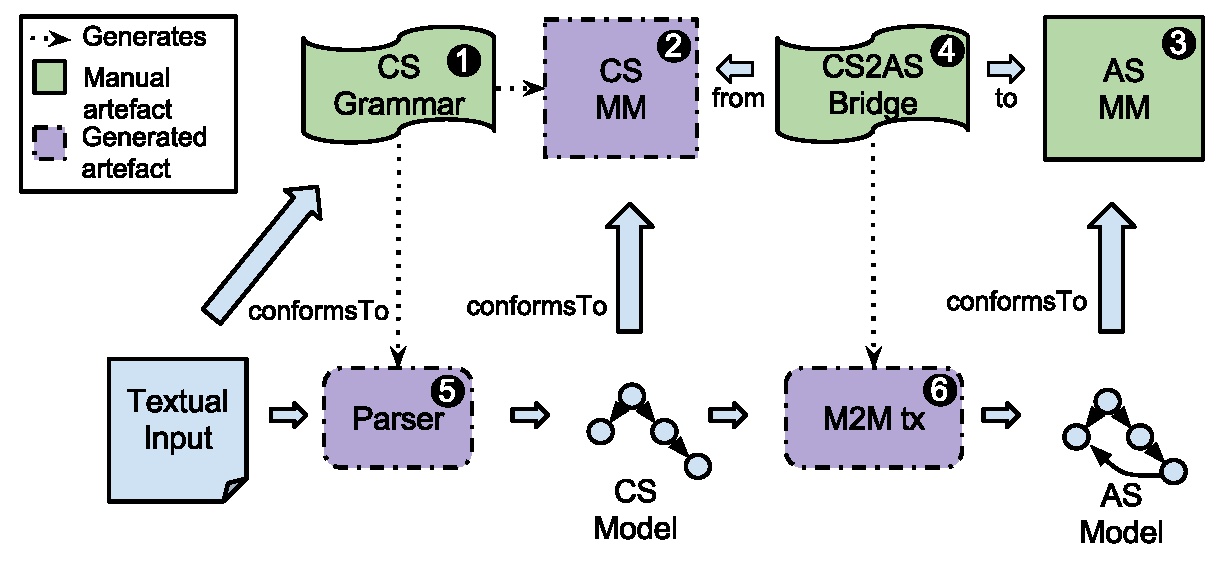
\includegraphics[width=\textwidth]{images/OverallApproach.pdf}
	\caption{Overall approach}
	\label{fig:OverallApproach}
\end{figure}
	
With the proposed approach we operate in the modelware technological space. The significant parsing concerns do not affect us and so we are not dependent on a particular parser and/or language workbench technology.  % We just rely on the existence of a CS meta-model (generated or not) and the existence of a parser which will provide the CS models for a given input. 
For example, Xtext (and ANTLR~\cite{antlrOnline} based parsers) are suitable for this approach. More generally, any underlying parser produces CS models conforming to a meta-model could be used. We could therefore use IMP~\cite{charles2009imp} (and LPG~\cite{lpgOnline} based parsers). % The description between the CS and AS should certainly be parser agnostic.

\subsection{CS2AS External DSTL}
\label{subsec:dstl}

We propose a new external DSTL for the CS2AS definition~\ding{205} in Fig.~\ref{fig:OverallApproach}. We use a new DSTL rather than an existing M2M transformation language, to provide a more concise declarative language in this domain. The DSTL reuses Essential OCL as the expressions language. The following characteristics led us to define it as a DSTL:

\textbf{One input and output domain}. The model transformations involves just one source input domain and one target output domain. Each domain which may comprise several meta-models. There is no need to support in-place transformations.

\textbf{Specific name resolution related constructs}. We add specific constructs to define name resolution in a declarative manner.

\textbf{Specific disambiguation rules}. The CS disambiguation concern is separated by providing a dedicated declarative section to specify the disambiguation rules that drive AS element construction.


%Due to limited space, we focus on exposing the features that address the issues identified in Section~\ref{sec:problem}, taking the example introduced in Section~\ref{subsec:motivation} to show concrete excerpts.

The DSTL consists of four different sections: \textit{helpers}, \textit{mappings}, \textit{name resolution} and \textit{disambiguation}. Each addresses a particular concern of the process of describing CS2AS bridges, and they are introduced below.

\textbf{Helpers.}
The helpers section provides reusable functionality in the form of helper operations. For instance, Listing~\ref{lst:HelpersExcerpt} depicts a declaration of a helper operation that retrieves the parent element of a \textit{NameExpCS} as another \textit{NameExpCS}. When the parent element is either \textit{null} or a non-\textit{NameExpCS}, \textit{null} is returned.

\begin{lstlisting}[caption=Helpers section excerpt, label=lst:HelpersExcerpt, language=CS2AS]
helpers {
  NameExpCS::parentAsNameExp() : NameExpCS[?] := 
      let container = self.oclContainer()
      in if container.oclIsKindOf(NameExpCS)
         then container.oclAsType(NameExpCS)
         else null endif  }
\end{lstlisting} 

\textbf{Mappings.}
The \textit{mappings} section is the main part of the DSTL. The mappings declare how AS outputs are created and initialized from CS inputs. The DSTL includes the basics of declarative M2M transformation languages\cite{czarnecki2003classification}.

%Listing~\ref{lst:MappingsExcerpt} depicts an excerpt for our example. %Line 2 declares that a \textit{PropertyCallExp} might be created from a \textit{NameExpCS}. Line 3 refers to a disambiguation rule, and it will be explained later on. % Here, the reader just need to know that they act as mapping guards. 
%Line 4, will declare how \textit{PropertyCallExp::ownedSource} property is computed. Firstly, it might be noticed that the helper we introduced before is invoked on \textit{self}. The \textit{self} keyword always refers to the contextual CS element, source of the mapping, and it might normally be removed. If we syntactically check that the \textit{NameExpCS} is not navigated (i.e. it's not a nested \textit{NameExpCS}), a \textit{VariableExp} is created referring to the implicit 'self' Variable, otherwise we are interestesd in the AS element created from the parent \textit{NameExpCS} element. The latter is declared with the first of the special expressions added to OCL in our DSTL: \textbf{resolve}. A resolve expression simply returns, by the means of traces information, the AS element created from a CS one (source of that resolve expression). Lines 7 and 11, include the second (and last) kind of special expression: \textbf{lookup}. They are explained later on. In line 12, we see how cross-references can be established by making use of the expressions language.

\begin{lstlisting}[float, caption=Mappings section excerpt, label=lst:MappingsExcerpt, language=CS2AS]
mappings {
  map PropertyCallExp from NameExpCS 
    when nameRefersAProperty {
      ownedSource := let parent = self.parentAsNameExp()
                     in if parent = null
                       then VariableExp {
                         referredVariable = trace.lookup(Variable, 'self'); }
                       else parent.trace;
                       endif
      property := trace.lookupFrom(Property, sName, trace.ownedSource.type)
      type := trace.property.type }}
\end{lstlisting}

Listing~\ref{lst:MappingsExcerpt} depicts an excerpt for our example; we highlight the relevant features. Line 3 refers to a disambiguation rule that is specified in the \textit{disambiguation} section (explained later). Lines 7, 8, 10 and 11 make use of \textit{trace} expressions, which let us access the AS domain from CS elements. Lines 7 and 10 make use of \textit{lookup} expressions to compute name resolution based cross-references (more details later). 

The \textit{mappings} section addresses complex CS2AS mappings like that required by our example. The use of OCL supports  complex computation and full navigation of the CS and AS models. % In this case, the input elements involved in the mappings are a NameExpCS and a SimpleNameCS. The output elements that might be created by this mapping are a PropertyCallExp and a VariableExp.

%Although  needed in our simple example, we explain another DSTL feature required by the comparative study presented in Section~\ref{subsec:featuresComparison}. The mappings exposed before, allow us to the declare how AS elements are created from CS ones, establishing a trace link between one source CS element and the target AS. These trace links might be used by resolve expressions to access the AS domain from the CS one. Sometimes, We might want to access the AS domain from CS elements, even though no particular AS element is created. %This scenario is normally found when we have CS elements conceived to create cross-references in the AS, for instance when have a name used to look up a type in the AS. 
%The syntax to support this kind of declarations can be depicted by Listing~\ref{lst:MappingsExcerpt2}.

%\begin{lstlisting}[caption=Mappings section excerpt, label=lst:MappingsExcerpt2, language=CS2AS]
%mappings {
%  map Type from TypeRefCS :=
%     resolve.lookup(Type, pathName)
%}
%\end{lstlisting}

\textbf{Name resolution.}
The third section of the DSTL specifies how names are resolved. % to create cross-references in the AS models. Name resolution is a so common activity, even in simple modeling languages, that the DSTL incorporates dedicated syntax for it. 
Explaining the full capabilities of the language would merit its own paper. We therefore focus on what is required to explain name resolution in our example: in particular, how a \textit{Property} might be located to resolve the \textit{PropertyCallExp::referredProperty} cross-reference.

%Name resolution consists of performing a lookup activity from an AS element with the aim of finding another AS (named) element located somewhere else in the AS model. The input of this lookup activity is normally CS related information (e.g. a name), whilst the output is the desired AS model, target of a  cross-reference. In our DSTL we identify three kind of named element lookups (i.e three different name resolution protocols): \textbf{unqualified}, \textbf{qualified} and \textbf{exported} named element lookups. 
%In the name resolution section, it will be declared how the different types of AS elements will contribute named elements for the different kind of name lookups.


\begin{lstlisting}[caption=Basic name resolution declaration for \textit{Property} elements lookup., label=lst:unqualifiedLookup, language=CS2AS]
nameresolution {
  Property { 
    named-element name-property name; }
  Class {
    for all-children -- scopes can be configured for all-children elements
      nested-scope ownedProperties;
    exports ownedProperties; }}
\end{lstlisting}

Listing~\ref{lst:unqualifiedLookup} shows the solution for the simple case. We firstly identify \textit{Property} as a named element, the target of name-based lookups (lines 2-3). Basic unqualified named element lookups are based on the concept of lookup environments (scopes) propagation (Clause 9.4 of~\cite{omg2014ocl}). They are detailed in our previous work~\cite{sanchez2015oclCS2AS}. In our example, we declare how \textit{Properties} are contributed to lookup scopes. In this case, it is done by the owning \textit{Class} (Lines 5-6). Since a property name might occlude others defined in outer scopes, we use the \textbf{\textit{nested-scope}} keyword. 

Named elements might be the target of lookups out of the scope of the element that performs the lookup. For instance, a \textit{PropertyCallExp} may refer to a \textit{Property} of a \textit{Class} that is not the \textit{Class} defining the expression's scope. Thus, we also declare that a \textit{Class} \textbf{exports} its owned \textit{Properties} (line 7). 

Finally, we explain how name-based lookups are linked with the mappings section. In Listing~\ref{lst:MappingsExcerpt}, we remarked on two new expressions that enhance OCL: \textbf{lookup} expressions (line 7) are used to declare a named element lookup in the current scope. They require the target element type and additional input information (the string \textit{'self'}, in that example); \textbf{lookupFrom} (line 10) expressions are used to look up \textbf{exported} elements. They require another parameter indicating from which element the lookup is performed (the \textit{type} of the \textit{ownedSource}, in that example).


%In a first place, \textbf{Unqualified named element lookups} are explained. It simply consists of locating AS named elements which are in the scope (also known as environment in~\cite{omg2014ocl}) computed for the AS element which performs the name-based lookup. A scope is conceptually a map of name-to-named-element exposing all the candidate AS named elements target of a name-based lookup. It's always declared in a top-down fashion. This means that for a particular AS element we declare how the scope will be propagated to its children AS elements. By default, the scope of the AS element parent will be propagated as it is to all children element. The DSTL name resolution section allows then to declare how a scope is particularly configured to its children elements, which normally implies adding adequate named elements to the scope. The scopes can be nested, allowing to occlude named elements (with the same name) already existing in outer scopes.

%\begin{lstlisting}[caption=Basic name resolution declaration for \textit{Property} elements lookup., label=lst:unqualifiedLookup, language=CS2AS]
%nameresolution {
%  Property { 
%    named-element name-property name;
%  }
%  Class {
%    for all-children // It might be removed, all-children is the default
%      nested-scope ownedProperties, ownedOperations;
%  }
%}
%\end{lstlisting}

%Listing~\ref{lst:unqualifiedLookup} shows a first excerpt to declare the name resolution related to a \textit{Property}. At Line 4, we declare that \textit{Property} elements are target of a name resolution, including which is the property involved in the name-based lookup\footnote{OCL AS offers a common NamedElement::name property. We might globally declare it as such to avoid to write the name-property declaration for every possible AS element participating in the name resolution}.

%We also need to declare how \textit{Property} elements are contributed to lookup scopes. In this case, \textit{Class} elements are the adequate AS elements to deal with. So at lines 6 and 7, we declare that a Class propagates for all its children a nested scope, which includes all the \textit{Property} elements accessed via the \textit{ownedProperties} expression (\textit{ownedOperations} is for operations lookup purposes). 

%Note the usage of OCL expressions to do the contributions to the scope. They let us declare more complex navigations through the AS to locate the required named elements. This is actually required for another requisite: we also have to consider the properties of any super \textit{Class}. Listing~\ref{lst:occludingSuperProperties} shows a possible declaration to comply with that requisite. Note the \textit{occluding} keyword to create an additional nested scope, which allows us to occlude the properties of super classes \textit{Property} elements in favour of those owned by the \textit{Class} element.

%\begin{lstlisting}[caption=Contributing \textit{superClasses Property} elements, label=lst:occludingSuperProperties, language=CS2AS]
%nameresolution {
%  Class { 
%    for all-children
%      nested-scope ownedProperties,ownedOperations
%        occluding let allSuperClasses = self->closure(superClass)
%                  in allSuperClasses.ownedProperties
%                      ->includingAll(allSuperClasses.ownedOperations);
%  }
%}
%\end{lstlisting}

%In a second place, we need to introduce the \textbf{Exported named element lookups}. Unqualified named element lookups rely on a scope propagation based on the containment hierarchy (from-parent-to-children) of an element, so that an specific \textit{Property} element of a given \textit{Class} element might be found from any \textit{PropertyCallExp} which is directly or indirectly contained by that \textit{Class} element. However, we might often find that the wanted \textit{Property} element doesn't belong to the \textit{Class} element containing the call expression. For instance, in our example we want to access the property 'y' of the \textit{Class} corresponding to the type of 'x' (the source expression).

%Listing~\ref{lst:qualifiedLookup} depicts these situations are tackled. We want to declare which are the candidate named elements to be looked up (i.e. exported named elements), when the name-based lookup is performed from an AS element which is out of the scope of contributing element (i.e. the former is not contained by the latter). 

%\begin{lstlisting}[caption=Contributing \textit{superClasses Property} elements, label=lst:qualifiedLookup, language=CS2AS]
%nameresolution {
%  Class { 
%    ...
%    exports ownedProperties,ownedOperations
%      occluding let allSuperClasses = self->closure(superClass)
%                in allSuperClasses.ownedProperties
%                    ->includingAll(allSuperClasses.ownedOperations);
%  }
%}
%\end{lstlisting}

%Note that the named element contributions for the two different lookup protocols don't have to be the same. For instance, if we were working with a Java meta-model we would like to declare that for unqualified named element lookups, public and protected class members of super classes are contributed, whereas for exported named element lookups, only public class members of super classes must be considered, instead.

%Finally, we explain how the name resolution definition is linked with the mappings section. The set of OCL expressions is enhanced with two dedicated call expressions, to express that a lookup activity needs to be performed. The Figure~\ref{lst:MappingsExcerpt} we mentioned before, contains usage of both:

%\begin{itemize}
%	\item At line 7, a \textbf{lookup} call expression performs an unqualified named element lookup. It passes two arguments: the first is the kind of named element to look up; the second is the CS information used as input (e.g. a name).
%	\item At line 11, a \textbf{lookupFrom} call expression performs an exported named element lookup. It passes three arguments: the first is the kind of named element to look up, the second is an expression which evaluates to the actual element from which the exported named element lookup will be performed; the third is the CS information used as input (e.g. a name).
%\end{itemize}

\textbf{Disambiguation.}
The \textit{disambiguation} section of the DSTL declares CS disambiguation rules which can be referred to by mappings declared in the \textit{mappings} section. These disambiguation rules act as a guard for the referring mapping. %, so that we can drive the AS element creation based on some specific disambiguation rules. 
Listing~\ref{lst:disambiguationExcerpt} shows an example of disambiguation rules required by our introductory example.

\begin{lstlisting}[caption=CS disambiguation rules, label=lst:disambiguationExcerpt, language=CS2AS]
disambiguation {
  NameExpCS { 
    nameRefersAVariable := 
      let asParent = oclContainer().trace
      in asParent.lookup(Variable, sName) <> null;
    nameRefersAProperty := 
      let csParent = parentAsNameExp(),
          asParent = oclContainer().trace
      in if parentNameExpCS = null
         then asParent.lookup(Property, sName) <> null
         else asParent.lookupFrom(Property, csParent.trace.type, sName) <> null
         endif; }}
\end{lstlisting}

%Line 2, simply refers to the CS element (NameExpCS) which requires some disambiguation rules. In lines 3 and 6, we declare two disambiguation rules which will drive what AS element must be created from a particular NameExpCS: either a VariableExp element or a PropertyCallExp one.

%A disambiguation rule consists of a left hand side identifier, and a right hand side boolean valued OCL expression. The identifier, can be referred from a mapping rule by the means of the \textit{when} keyword  as we previously showed in Listing~\ref{lst:MappingsExcerpt}. The OCL expression might access CS information from the contextual CS element, even make use of resolve expressions to access the AS domain. For instance, in our example we require name-based lookups in the AS. % That said, it should be taken into account that disambiguation rules evaluation precedes the corresponding AS creation. Therefore, disambiguation rules which require AS information, must access the AS domain from its parent CS element, as exposed in lines 4 and 8 from Listing~\ref{lst:disambiguationExcerpt}.

Our DSTL separates the disambiguation rules from the mappings section. This lets us solve a typical issue in declarative transformation languages where mappings applied to the same input type contain non-exclusive guards (two guards might evaluate to true).
%Finally, we clarify the last issue. In CS disambiguation scenarios, we normally find different mappings applying to the same CS element, and referring to their corresponding disambiguation rules. It might happen that two or more disambiguation rules of those mappings evaluate to true for a particular CS element, provoking a new dilemma about which mapping rule should be executed.
For instance, in our example, \textit{'x'} might be both a variable to refer in that particular expression scope, \textit{and} a property of the \textit{'self'} variable. In order to address this issue and keep the mappings section declarative, we enhance the semantics of the disambiguation section so that the order in which the disambiguation rules are defined is significant: the first disambiguation rule that applies for a particular CS element is used. In our example, and providing the mentioned conflict, \textit{'x'} disambiguates to a \textit{VariableExp}, rather than a \textit{PropertyCallExp}, since the \textit{nameRefersAVariable} disambiguation rule is defined first.

\subsection{Implementation}

The DSTL has been prototyped using Xtext. The corresponding Eclipse plugins are publicly available\footnote{\url{https://github.com/adolfosbh/cs2as}}. The implementation does not include an M2M transformation engine capable to execute instances of the DSTL, rather it contains an Xtend-based~\cite{xtend} code generator\footnote{Implementation details about the generator are not included in this paper} that generates a set of Complete OCL files conforming to the OCL-based internal DSL described in our previous work~\cite{sanchez2015oclCS2AS}. As explained in \cite{sanchez2015oclCS2AS}, the actual CS2AS transformation execution is performed by a generated Java class that uses the Eclipse Modeling Framework and Ecore meta-models to transform CS models to AS models.

\section{Related Work}
\label{sec:relatedWork}

We now discuss how our approach relates to previous work. Space constraints prevent a detailed comparison with the very many tools that provide partial support to the problems
identified in this paper, including TEF\cite{scheidgen2008tef}, Spoofax\cite{kats2010spoofax} and Monticore\cite{krahn2010monticore}. %If we have a look to previous Language Workbench Challenges, we might find a bunch of candidates which would merit a mention.
%To cite a few of them: Xtext\cite{eysholdt2010Xtext}, , etc.
%We firstly highlight that this paper is a continuation of our previous work~\cite{sanchez2015oclCS2AS}, in which we admitted the need for an external DSL to declare CS2AS bridges.
The state-of-the-art related to this research is Gra2mol~\cite{canovas2012gra2mol} for which we include a detailed comparative study (Sect.~\ref{sec:gra2mol}). Here, we discuss two particular language workbenches in more detail: Xtext, because it has motivated this research and we aim to integrate with it; and Spoofax, whose  NaBL\cite{konat2013decNameRes} sub-language has been a source of inspiration of a part of our DSTL. 

\subsection{Xtext}

The introduction mentioned some of the limitations of Xtext; we now relate the challenges from Sect.~\ref{sec:problem} to Xtext's capabilities.

\textbf{Challenge 1}. Although Xtext grammars provide mechanisms to bridge the CS and AS of a language, as soon as we move away from simple DSLs to those that require M-N mappings, Xtext is insufficient.

\textbf{Challenge 2}. Xtext grammars support name resolution for cross-references in the AS models. They do not support derived resolution such as the types of OCL expressions.

\textbf{Challenge 3}. Xtext grammars resolve names using simple implicit scoping rules. More complex scoping scenarios requires customized code.

\textbf{Challenge 4}. Xtext provides no way to declare CS disambiguation rules.

%\textbf{Discussion.} Although the language specification artefacts (i.e the Xtext grammars) are not enough to describe the CS2AS bridge of languages like OCL, and given the powerful customizable framework it provides, creating tools for OCL using Xtext is still plausible. For instance, Eclipse OCL~\cite{eclipseOclOnline}, provides an Xtext-based tooling (parser, editor) capable of consuming OCL textual inputs and producing models conforming to the AS.

%The taken approach is conceptually the same to the one we take for our solution. An Xtext grammar generates the parser capable of consuming textual OCL files and producing some CS models. Then, some hand-written Java components are in charge of processing those CS models in order to produce the AS ones. This java code conforms the executable artefact to bridge the OCL CS2AS gap.

%Xtext takes EMF as its modelling framework, so the proposed prototype could complement Xtext to give better support to languages like OCL. By just creating an instance of our DSTL we should be able to capture the OCL CS2AS gap. The compiled and generated java transformation would then conform the executable artefact which might replace the current hand-written java code in charge of producing AS models from CS ones. As it is commented later on, future work.

\subsection{Spoofax}

%Spoofax is a language workbench to give support (e.g parsers, editors) to textual languages. Although it was not originally conceived to create models conforming to predefined meta-models, the goal might still be achieved by using additional facilities like Stratego/XT~\cite{visser2004stratego}. This assertion is demonstrated in this paper\cite{vanRest2013syncTextGraphEditors}, where the authors show how models can be edited by textual editors and graphical model editors in a synchronized way. Although they provide generic transformations so that they automatically generate a meta-model from their textual syntax definitions (as Xtext does), it's not clear how the general approach integrates with specific AS meta-model definitions. In any case, we might expect that specific Stratego/XT transformation might be specified between the AST produced by the parser (i.e what we refer as CS model), and a model conforming to an specific meta-model. Our DSTL would play the role of the general purpose programs transformation language Stratego/XT.

%\textbf{Discussion.} The main difference we can highlight between our DSTL and the different Spoofax languages is the following. As it occurs with Xtext, the name resolution activity is integrated in the parsing activity. Name resolution descriptions (using NaBL\cite{konat2013decNameRes} are only aware of the grammar descriptions (using SDF\cite{kats2010sdf}). This causes two main problems:
%\begin{itemize}
%	\item Name-based cross referencing is limited to refer elements that were parsed from the text. In other words, we could not create AS models referencing external AS models (e.g. a library AS model with no CS). 
%	\item In the required Stratego transformation, we can't declare CS disambiguation rules relying on name resolution. This means that any CS ambiguity resolution that requires name resolution and AS model information, can't be adequately described in Spoofax. 
%\end{itemize}

%Our approach postpones name resolution based cross-referencing (and any AS model cross-reference) to a further step, allowing name resolution based declarations to be adequately reused by the CS2AS mappings.

%NaBL has inspired some features of the name resolution section of our DSTL. Getting into details about them is beyond the goal of this paper. The real contribution resides in integrating a NaBL-like language as part of the DSTL.

%Given that Spoofax can work with EMF, our solution might be used within modelling languages defined with Spoofax. That said, there is not yet implementation to integrate the CS2AS descriptions (e.g. name resolution) with the different Spoofax editor services.

Spoofax is a language workbench to give support -- e.g parsers, editors -- to textual languages. Although it was not originally intended to create models, there is  work~\cite{vanRest2013syncTextGraphEditors} showing that Spoofax can be used for this purpose. We now relate the challenges from Sect.~\ref{sec:problem} to Spoofax capabilities.

\textbf{Challenge 1}. Past Spoofax work~\cite{vanRest2013syncTextGraphEditors} to generate meta-models from grammars suffers from the same limitations as Xtext (above). However, Stratego/XT \cite{visser2004stratego} can be used within Spoofax to address this challenge. Building on its foundations, we can define transformations from AST elements (i.e., the CS model) produced by a parser into an AS model.

\textbf{Challenge 2}. Stratego/XT can resolve cross-references in the AS model.

\textbf{Challenge 3}. Spoofax offers a declarative name resolution language (NaBL \cite{konat2013decNameRes}). However, the name resolution descriptions are only aware of the grammar descriptions (SDF~\cite{kats2010sdf}). Cross-references are set when producing the initial AST obtained from the parser. This inhibits cross-references to external AS models -- e.g. an AS model with no CS. In the case of OCL, many of the external (meta-)models on which OCL queries operate do not necessarily relate to any textual CS at all.

\textbf{Challenge 4}. Stratego/XT specifies disambiguation rules using \textit{strategy expressions}. There is no convenient way to declare CS disambiguation rules relying on name resolution.

\section{Gra2Mol: Comparative Study}
\label{sec:gra2mol}

We consider Gra2Mol as the-state-of-the-art related to this work. Although it was originally intended as a text-to-model tool for software modernization, their DSTL fits in the same scope and objective we present in this paper. To better assess how our proposed DSTL contributes to the field, we present a comparative study with Gra2Mol. The study consists of a qualitative evaluation in terms of features/capabilities and a quantitative evaluation in terms of performance.

\subsection{Qualitative Study}
\label{subsec:featuresComparison}

In this section we compare Gra2Mol and our DSTL in terms of their features and capabilities. Due to restricted space, we focus on relevant differences.
%Firstly, as we did with the related work discussed in Section~\ref{sec:relatedWork}, we discuss how gra2mol can deal with the issues presented in Section~\ref{sec:problem}.
%\begin{itemize}
%	\item \textbf{Issue 1}. 
%	\item \textbf{Issue 2}. 
%	\item \textbf{Issue 3}. 
%	\item \textbf{Issue 4}.
%\end{itemize}

%\textbf{Technology dependency.} The proposed DSTL is parser technology agnostic. It might be used with classic parser generators (e.g ANTLR, LPG) or modern language workbenches (Xtext, Spoofax). The main requirement is that the output of the parser is a model conforming to a meta-model (CS one), and the current solution depends on the Eclipse Modelling Framework. 

%Gra2Mol works on top the same modelling framework, and the main difference is that our DSTL operates on any arbitrary (possibly heterogeneous) CS meta-model, whereas Gra2Mol works on a unique (homogeneous) CS meta-model (called CST meta-model in~\cite{canovas2012gra2mol}) they define. This would prevent to seamlessly integrate Gra2Mol in tools generated by a language workbench like Xtext. Although this kind of integrations was not a goal of Gra2Mol at all, it's worthy to remark that the presented prototype fits better that purpose. 

%\textbf{Declarative nature.} Both languages are similarly declarative, which makes CS2AS definitions clear and concise. However, declarative languages require well designed execution engines, otherwise it might negatively impact performance. A quantitative study about performance will be presented in Section~\ref{subsec:benchmark}.

\textbf{Query language.} Gra2Mol is based on a tailored structure-shy (like XPath) query language, and our DSTL is based on the statically typed OCL. %Despite planned feature additions in OCL (e.g. safe naviation [?]), 
The Gra2Mol query language is less verbose and more concise than OCL; thus,  Gra2Mol instances tend to be smaller. However, Gra2Mol navigation operators are based on accessing children elements. This forces\footnote{Gra2Mol has a language extension mechanism to introduce new operators, which could be used to improve the default built-in functionality.} the declaration of deep navigations from the root element, whenever the information is not contained by a given CS element. This leads to performance penalties, because the operators are not as fast as a simple oclContainer() call. Also, the Gra2Mol query language is designed to work strictly on CS models. This has some advantages (e.g., conciseness) compared with our DSTL, because the latter requires usage of \textit{trace} expressions to access the AS domain. However, navigating the AS domain (graphs) from the CS one (trees) provides more concise and/or less expensive navigations to retrieve some particular AS information (e.g. querying the type -- a cross-reference -- of a particular expression). More importantly, focusing on CS navigations prevents CS2AS transformations from working with external AS models (e.g. a library model with no CS).

%	\item A statically typed language like OCL enables usage of a wide range of techniques based on static analysis. A textual editor can provide better content-assist facilities. Execution engines can provide good execution schedules for the transformation based on the dependency analysis of mappings and the involved expressions. When the grammar evolves, and so does CS meta-model, tools can help in the migration of existing CS2AS bridges, etc.

\textbf{Name resolution.} Name-based cross-references are declared in Gra2Mol as another model query. These queries are described as direct searches that consider where the target element is located in the model. Model queries get significantly complicated when simulating lookup scopes. In complex languages like OCL, the declarative nature of our \textit{nameresolution} section makes name-based cross-reference declarations concise.

%In our DSTL we introduce a dedicated declarative name resolution description, separating this particular concern in its own section. Lookup scopes are easily declared in the language and  now we don't have to elaborate how to reach a particular named element. Instead, we have to focus on how they are contributed to the lookup scopes. These contributions are usually easy to identify since the general case is that a named element is contributed to the lookup scope by its owner (e.g properties and operations are contributed by the owning class. Classes are contributed by the owning package. A let variable is contributed by the owning let expression etc.). For abnormal cases, more complex OCL expressions can be used to configure the scope contributions.

%\textbf{Disambiguation.} CS disambiguation scenarios can be similarly described with Gra2Mol by the means of rule filtering expressions applied to different rules working on the same grammar concept. These filtering expressions act as traditional M2M transformation mapping guards. The only drawback we have identified is related to the following imposition of their language: "If two or more conforming rules exist, their filter conditions must be exclusive, since only one of them can be applied"~\cite{canovas2012gra2mol}. The particular disambiguation scenario explained in Section~\ref{subsec:dstl}, is a case where two rules are applied to the same input element, whose disambiguation rules might both apply. There is still a workaround to this situation with Gra2Mol. To make the filtering expressions be exclusive, we would have to add additional condition checks related to what the other filtering expression is checking. However, we not are not only losing the declarative nature of mappings, but also the number of additional conditions will undesirably grow, as the number of potential rules with non-exclusive filtering expression does.

\textbf{Disambiguation rules.} Separating the disambiguation rules away from the mapping declarations provides additional semantics and overcomes a Gra2Mol limitation~\cite{canovas2012gra2mol}: ``If two or more conforming rules exist, their filter conditions must be exclusive, since only one of them can be applied". This limitation prevents a simple Gra2Mol solution to our introductory `x.y' example.

\textbf{Front-end coupling.} Our DSTL is not coupled to a parser technology or language workbench. The Gra2Mol transformation interpreter is coupled to a homogeneous CS meta-model they provide, which is incompatible  with Xtext grammars; more generally, integrating Gra2Mol with a language workbench like Xtext is impractical.

%In our DSTL we separate the disambiguation rules, in its own section, away from the actual referred mapping. With a policy based on disambiguation rules ordering (first matched), we can better declare how non-exclusive disambiguation rules are resolved. Since we move the disambiguation rules definition away from the mappings, the declarative nature of the mappings section is preserved.

%\textbf{Rule inheritance.} Gra2Mol provides rule inheritance mechanisms in order to create rules that declare queries and mappings common to and to be reused by other rules. They are called mixin rules, and they require that (input and output element) types of the extending rule (sub-rule) conform to the types of the extended one (super-rule). You must explicitly state the name of mixin rule that a specific rule inherits.

%For the proposed DSTL, as long as the involved (input and output) types conform [? ] to the types of any other, rule inheritance is assumed between them. This decision would imply additional work to be done by the compiler, but it let us not to make the different rules identifiable by name (improvement conciseness). For completeness, we permit redefinition (override) of property initializations, so that a sub-rule can respecify any property initialization done by any of its super-rules. This particular rule inheritance mechanism is not currently implemented by the compiler, so we currently don't support execution of transformation relying on the proposed rule inheritance mechanism.

%\textbf{Language expressiveness.} By the means of the helpers section, and the expressiveness of OCL, the user can declare complex functions required to perform a particular computuation of an AS element property. Although this is not the case for the Gra2Mol built-in language, the tool provides an extension mechanism tp add new mapping and query operators. These can be conceived and implemented as a Java black boxes, complying with the expressiveness requirement. Our DSTL doesn't currently support black box operations, so our limits are set by the OCL language expressiveness.

%\textbf{Additional Gra2Mol language constructs}. We finally show how additional language capability of Gra2Mol might be supported with the proposed DSTL. Gra2Mol allows to define special rules, called skip rules, to give support to a particular issue that turns up when working with with LL-grammars. In particular, when some trivial operators precedence are specified via grammar rules. 

%The problem can be summarized as follows (issue extended explanation and gra2mol solution might be found in \cite{canovas2012gra2mol}). Listing~\ref{lst:andExp} depicts an Xtext grammar rule corresponding to a Java 'or' logical expression.

%\begin{lstlisting}[caption= Grammar rule of an 'or' logical expression in Java, label=lst:andExp, language=CS2AS]
%OrExpCS:
%  mandatoryExp=AndExpCS ('||' optionalExps+=AndExpCS)* ;
%\end{lstlisting}

%When defining the CS2AS mapping for this CS element, we find the issue that OrExpCS should be mapped to one (or many) 'or' logical expression(s), but only in the case that (at least) one 'or' logical operator has been found. In principle, by the means of disambiguation rules we could declare that 'or' logical expressions should be created whenever \textit{OrExpCS::optionalExps} is no empty. However, we don't want to create any new AS element when no 'or' logical operator has been processed. In this case, we must make use of the second kind of CS2AS mapping definition we explained for the DSTL mappings section, in which we declare that the CS element will be mapped to another AS element, rather than create a new one. See Listing~\ref{lst:orExpCSmapping}

%\begin{lstlisting}[caption=CS Disambiguation Rules, label=lst:orExpCSmapping, language=CS2AS]
%map OrExpression from OrExpCS when orOpProcessed {/*props computation*/};
%map Expression from OrExpCS when orOpNotProcessed := mandatoryExp.resolve; 
%\end{lstlisting}

\subsection{Quantitative Study}
\label{subsec:benchmark}

The quantitative study consists of an experiment based on obtaining execution time measurements for both Gra2Mol and our prototype when executing CS2AS transformations. We focus on execution time because we aim to integrate these CS2AS transformations in textual editors, where too-slow execution time is unacceptable.

Gra2Mol is publicly available with different ready-to-go examples. Our experiment replicates one of them with our prototype and performs a benchmark involving models of different size and/or topology.

\textbf{Example.} %Among the different examples that might be found in the gra2mol source code repository,
We have picked one of the published Gra2Mol examples that is simple enough to fit within our space constraints, that requires cross-references resolution, and provides models of varied topologies.

\begin{figure}[htbp]
   \captionsetup[subfigure]{labelformat=empty}
   \begin{SubFloat}[]{}
     \begin{minipage}{.5\textwidth}
		\begin{lstlisting}[label=lst:CompaniesCS, language=Xtext]
company :
  'company' STRING '{' 
  department* 
  '}' EOF;
department :
  'department' STRING '{' 
    department_manager
	department_employees
	department*
  '}';
department_manager :
  'manager' employee;
department_employees :
  ('employee' employee)*;
employee :
  STRING '{'
    'address' STRING
    'salary' FLOAT
    ('mentor' STRING)?
  '}';
		\end{lstlisting} 
      \end{minipage}
	\end{SubFloat}%
	\begin{SubFloat}{}
		\begin{minipage}{.5\textwidth}
		\centering
		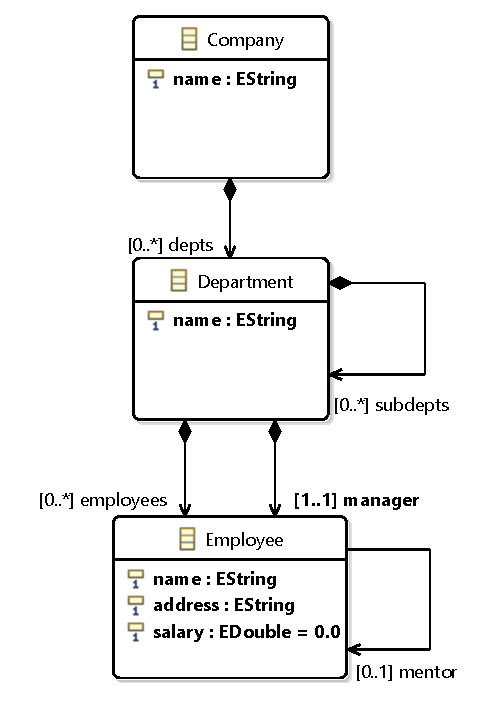
\includegraphics[scale=.5]{images/CompanyAS.pdf}
     	\end{minipage}
	\end{SubFloat}
	\caption{CS (left) and AS (right) of the target 101companies~\cite{favre2012101companies} example.}
	\label{fig:CompaniesExample}
\end{figure}

Figure~\ref{fig:CompaniesExample} shows the CS (ANTLR grammar) and AS (Ecore meta-model) of the modelling language, as defined by the target ``101 Companies`` example\footnote{\url{https://github.com/jlcanovas/gra2mol/tree/master/examples/Grammar2Model.examples.101companies}}~\cite{favre2012101companies}. The definition of lexical tokens has been intentionally omitted.



%For the experiment, we have replicated the example's grammar specification with an Xtext grammar, so that we can automatically generate the CS meta-model, to which our DSTL instance will refer.

%\begin{figure}[htbp]
%	\centering
%	\begin{subfigure}{0.65\textwidth}
%		\centering
%		\begin{lstlisting}[label=lst:ExampleGrammar, language=Xtext]
%company :
%  'company' name=STRING '{' 
%     deparment+=department* 
%  '}';
%department :
%  'department' name=STRING '{' 
%    department_manager=department_manager
%    department_employees=department_employees
%    deparment+= department*
%  '}';
%
%department_manager :
%  'manager' employee=employee;
%
%department_employees :
%  {department_employees}
%  ('employee' employee+=employee)* ;
%
%employee :
%  name=STRING '{'
%    'address' address=STRING
%    'salary' salary=FLOAT
%    ('mentor' mentor=STRING)?
%  '}';
%		\end{lstlisting} 
%	\end{subfigure}%
%	\begin{subfigure}{0.35\textwidth}
%		\centering
%		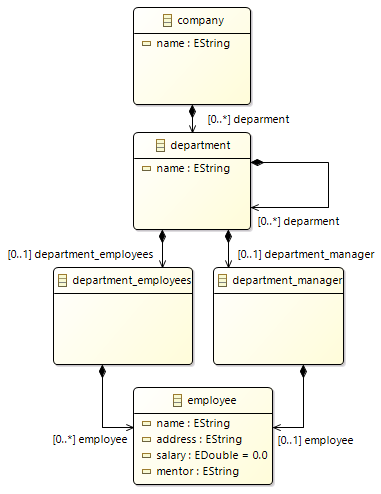
\includegraphics[scale=0.5]{images/CompaniesCS.png}
%	\end{subfigure}
%	\caption{Analogous Xtext grammar and corresponding CS meta-model.}
%	\label{fig:CompaniesCS}
%\end{figure}

\begin{figure}[htbp]
	\captionsetup[subfigure]{labelformat=empty}
	\centering
	%\begin{subfigure}{0.5\textwidth}
  	\begin{SubFloat}[]{}
  	  \begin{minipage}{0.45\textwidth}
		\centering
		\begin{lstlisting}[label=lst:Gra2MolExampleGrammar, language=gra2mol]
rule 'mapEmployee'
 from employee e
 to   Employee
 queries
  mElem : //#employee{STRING[0].eq(e.STRING[2])};
 mappings
  name    = removeQuotes e.STRING[0];
  address = removeQuotes e.STRING[1];
  salary  = e.FLOAT;
  mentor  = mElem;
end_rule
		\end{lstlisting} 
      \end{minipage}
    \end{SubFloat}	
	%\end{subfigure}%
	%\begin{subfigure}{0.5\textwidth}
  \hfill  
	\begin{SubFloat}[]{}
	  \begin{minipage}{0.45\textwidth}
		\centering
		\begin{lstlisting}[label=lst:DstlExampleGrammar, language=CS2AS]
mappings {
map as::Employee from employee {
  name := name;
  address := address;
  salary := salary;
  mentor := trace.lookup(Employee, mentor);}} 
nameresolution {
 Employee {
  named-element name-property name;}
 Company {
  nested-scope
   depts->closure(subdepts)
          ->collect(employees
          ->including(manager));}}
		\end{lstlisting}
      \end{minipage}
	\end{SubFloat}
 
    %\end{subfigure}
	\caption{CS2AS specification in Gra2Mol (left) and our DSTL (right).}
	\label{fig:CompaniesCS2AS}
\end{figure}


Figure~\ref{fig:CompaniesCS2AS} depicts side-by-side excerpts of the artefacts that show how the CS2AS bridge is specified within both approaches. There are numerous similarities between the CS2AS descriptions, where the main differences are in the model queries. Our DSTL isolates the name resolution concerns in its own section.


 %to resolve the \textit{Employee::mentor} cross-reference, in its own section. %That said, given the simple name resolution policy of the example, in which any employee might be mentor of any other employee, we can't note the benefits of the \textit{nameresolution} section. 

%Finally, Gra2Mol transformation requires additional facilities like \textit{removeQuotes}. The DSTL instance doesn't have to deal with them because the parser generated by Xtext does that job for us (when building the CS model). However, we have included an \textit{unquote()} helper, depicted by Listing~\ref{lst:unquoteHelper}, to simulate the additional work that the gra2mol transformation needs to perform (we aim to reduce threats to the experiment validity). 

%\begin{lstlisting}[caption= Unquote helper, label=lst:unquoteHelper, language=CS2AS]
%helpers {
%  String {
%    -- In the experiment, we will simulate an unquote function
%    -- We do not actually unquote, since the strings are already unquoted.
%    unquote() : String := self.substring(1,self.size());
%  }
%}
%\end{lstlisting} 
	
\textbf{Experiment Setup.} We now describe how the experiment is conducted. We ensure that the CS2AS transformation executions are correct by checking that the output models produced by both transformations are the same. 

We created a tailored model generator for the  example, configured by the following parameters:

$N_d$ : Number of (top level) departments in the company model.

$N_s$ : Number of subdepartments per department/subdepartment.

$N_e$ : Number of employees per department/subdepartment.

$D_s$ : Depth level of (sub)departments.


Element attributes are pseudo-randomly generated, whereas the \textit{Employee:: mentor} cross-reference is assigned to another random employee with a $0.5$ probability. The input models used in the experiment are characterized by Table~\ref{tbl:models}.

\begin{table}	
	\centering
	\caption{Experiment model characterization}
	\begin{tabular}{c||c|c|c|c|c|c}
	Model ID & Size (bytes) & Elements &  $N_d$ & $N_s$ & $N_e$ & $D_s$ \\
	\hline		
	$M_1$ & 1,238  & 22 & 3 & 0 & 3 & 1 \\
	$M_2$ & 6,105 & 97 & 3 & 3 & 4 & 2 \\
  	$M_3$ & 149,951 & 701 & 1 & 1 & 3 & 100 \\
	$M_4$ & 42,805 & 708 & 1 & 100 & 3 & 2 \\
	$M_5$ & 223,848 & 3061 & 4 & 4 & 5 & 4 \\
	$M_6$ & 1,018,254 & 11901 & 10 & 4 & 10 & 4 \\
	$M_7$ & 9,794,276 & 109341 & 10 & 5 & 10 & 5 \\
	%M8 & 1033341 & 10 & 9 & 10 & 5 \\
	\hline
	\end{tabular}
	\label{tbl:models}
\end{table}

The experiment consists of using both technologies to run the corresponding CS2AS transformation with each model. With the aim of easing repeatability, we have set up an experiment environment in the SHARE \cite{vanGorp2012share} platform\footnote{\url{http://share20.eu}}. The reader just needs to log in platform, and request access to the prepared virtual machine\footnote{\url{http://is.ieis.tue.nl/staff/pvgorp/share/?page=ConfigureNewSession&vdi=Ubuntu12LTS_CS2AS-DSTL---Experiments.vdi}}. When the access is granted, the user can connect to the remote virtual machine and access the system using \textit{Ubuntu} as user name, and \textit{reverse} as password. Additional information (README) about how to repeat the experiment, as well as more details about the environment can be found in the user desktop.
%\begin{itemize}
%  \item The JVM is configured to use a 4096MB heap.
%  \item To warm the JVM up prior to taking measurements, we will run 3000 times the main transformation execution code with $M_2$.
%  \item We then run and measure the main transformation execution 10 times with the specific model. The first measurement is discarded, having 9 data points.
%  \item Loading/saving models and parsing activities are excluded from the main transformation execution time.
%\end{itemize}

%We have modified\footnote{\url{https://github.com/adolfosbh/gra2mol/tree/icmt2016}} the Gra2Mol base code to obtain performance data from just the transformation execution (model loading/saving is thus not included). We have deactivated Gra2Mol debug/logging mode. The experiment for both technologies can be downloaded and replicated\footnote{\url{https://github.com/adolfosbh/cs2as/tree/icmt2016/org.xtext.example.companies}}\footnote{\url{https://github.com/adolfosbh/gra2mol/tree/icmt2016/examples/org.gra2mol.example.companies}}.

\textbf{Experiment Results.} We now present the results, including observations and discussion. Figure~\ref{fig:Results} summarizes the performance results. All the collected data and graphics are publicly available\footnote{\url{https://docs.google.com/spreadsheets/d/16aYZRdKiPOMA_z_85zfVFNLqPPe1XMvNsSdGIw8j7vw/edit?usp=sharing}}.

\begin{figure}[htbp]	
	\centering
	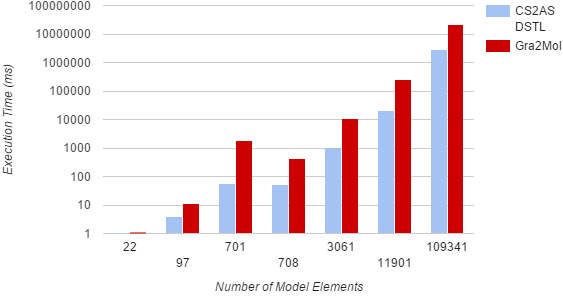
\includegraphics[scale=0.65]{images/Results.PNG}
	\caption{Experiment results: execution time.}
	\label{fig:Results}
\end{figure}

Overall, Gra2Mol is ten times slower than our prototype with respect to this example. There is an observed peak in performance when Gra2Mol deals with $M_3$ (701 model elements). It is unexpected, especially when comparing with $M_4$ (708 model elements) which has a similar number of model elements. If we look at the model parameters characterization from Table~\ref{tbl:models}, we identify two main differences: $M_3$ is a deep model, whereas $M_4$ is a wide one; Despite the similar number of model elements, $M_3$ is bigger in terms of size (149,951 vs 42,805 bytes). This is explained by the logic used by the model generator to assign names to model elements: the deeper the named element is inside the model, the longer the string for the corresponding name. These topology differences between $M_3$ and $M_4$, makes us conclude that model topology seriously impacts Gra2Mol performance, whereas this is not the case with our prototype.

 %% Explain

In terms of scalability, we observe that neither approach adequately scales (i.e bad performance results with big models). Some more comments about this limitation are given below.

%\section{Limitations and shortcomings}
%\label{sec:limitations}

%Creating these CS2AS bridges complementary to the grammar implies elaborating  a new artefact that will normally be as big as the grammar one. This is not ideal, and therefore our solution should be limited to languages that existing language workbenches can't straightforwardly cope with (i.e complex languages with a big gap between the CS and AS). That said, we will consider to apply other techniques (e.g. Flock [1] for meta-model evolution scenarios), so that the CS2AS specification artefacts size might be significantly reduced.

\textbf{Limitations.} Neither Gra2Mol nor our prototype scaled proportionately; we repeated the experiment but we removed the computation of \textit{Employee::mentor} property from both transformations. For the latter, we also removed the model query required to compute that property. The results are depicted in Fig.~\ref{fig:Results2}.

\begin{figure}[htbp]	
	\centering
	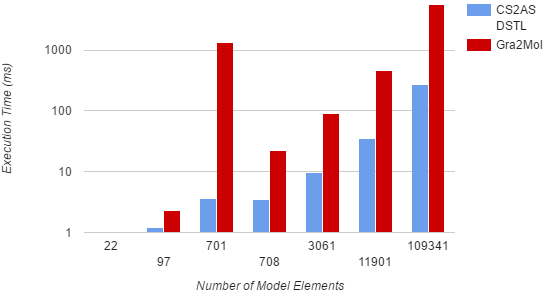
\includegraphics[scale=0.65]{images/Results2.PNG}
	\caption{Execution time when \textit{Employee::mentor} property is not computed.}
	\label{fig:Results2}
\end{figure}

We get more reasonable results that lead to the same previous conclusions. Additionally, we conclude that the bad performance results from the original experiment come from the expensive query to compute the \textit{Employee::mentor} property. In our prototype, when compiling to a Complete OCL document-based specification~\cite{sanchez2015oclCS2AS}, the name resolution behaviour is translated as a set of OCL operations. Given the name resolution defined for the example, the operational behaviour of these OCL operations implies traversing the whole model every time name resolution is required. In Gra2Mol the penalty is even worse (transformation of $M_7$ takes several hours), because the expensive traversal is performed even though a particular employee is not meant to have a mentor.

Although this an implementation issue, rather than a DSTL one, this is an important issue to address, and so we aim to address the missing re-computation cache in the near future.

\section{Remarks and future work}
\label{sec:futureWork}

In this paper, we have focused on textual CS. However, the proposed solution works in the modelware technological space. Thus, it might be used, for instance, with diagrammatic CS, as long as all the corresponding editing facilities produce a CS model (e.g figures, colours, etc.). This is something we aim to explore in future work, e.g., on editors for probabilistic state machines or flexible models.

In this paper, our DSTL establishes mappings from the CS towards the AS. However, many tools need to obtain the corresponding CS representation of an AS model, for instance, after a model refactoring. Although the traces between the CS and AS models are retained, the inverse transformation step is not currently supported. However, we see no immediate impediment to use the same DSTL to specify the opposite transformation. 

In this paper, we focused on the CS-to-AS transformation step. However, to add more value to the proposed language, additional tooling to better integrate with modern workbench languages is required. We have created some Xtext integration support, so that a generated editor benefits from an enhanced content assist produced from the name resolution description. Also, the generated outline view is enhanced to show the structure of the AS model rather than the CS model one. We want to polish and publish this work in the near future.

When comparing with Gra2Mol, we improved the DSTL's declarative nature by incorporating a NaBL-like sub-language to support name resolution based cross references. We could improve the DSTL further by incorporating an XSemantics-like~\cite{bettini2013xsemantics} sub-language to support type system resolution based cross references.

\section{Conclusions}
\label{sec:conclusions}

We have proposed a new DSTL to bridge the CS and AS of languages, in particular, those whose CS is textual and specified by a grammar, and whose AS is specified by an established meta-model. We have justified the need for this language by showing some specific challenges that arise when the CS and AS bridge is non-trivial, in particular in OCL. The proposed solution operates in the modelware technological space, and hence does not commit to a particular parser technology or language workbench. 

After a qualitative comparison with Gra2Mol (state-of-the-art), we showed an experiment whose results provide evidence that our prototype outperforms -- in terms of execution time -- Gra2Mol (in the example, ten times fold).

Although there currently are limitations, the proposed solution makes a substantial step towards providing the required support for complex textual modelling languages (e.g OCL), by means of specification artefacts such as grammars, meta-models and domain specific transformations.

\vspace*{1mm}
\textbf{Acknowledgement.}
We gratefully acknowledge the support of the UK Engineering and Physical Sciences Research Council, via the LSCITS initiative, and Javier Lu\'{i}s C\'{a}novas Izquierdo (Gra2Mol) and Pieter Van Gorp (SHARE) for the technical support required to produce the results exposed in this paper.

\bibliographystyle{unsrt}
\bibliography{icmt2016}

\end{document}